\section{Can the input be trusted? A controlled null result}
\label{sec:prep-null}

\begin{figure}[!htb]
\centering
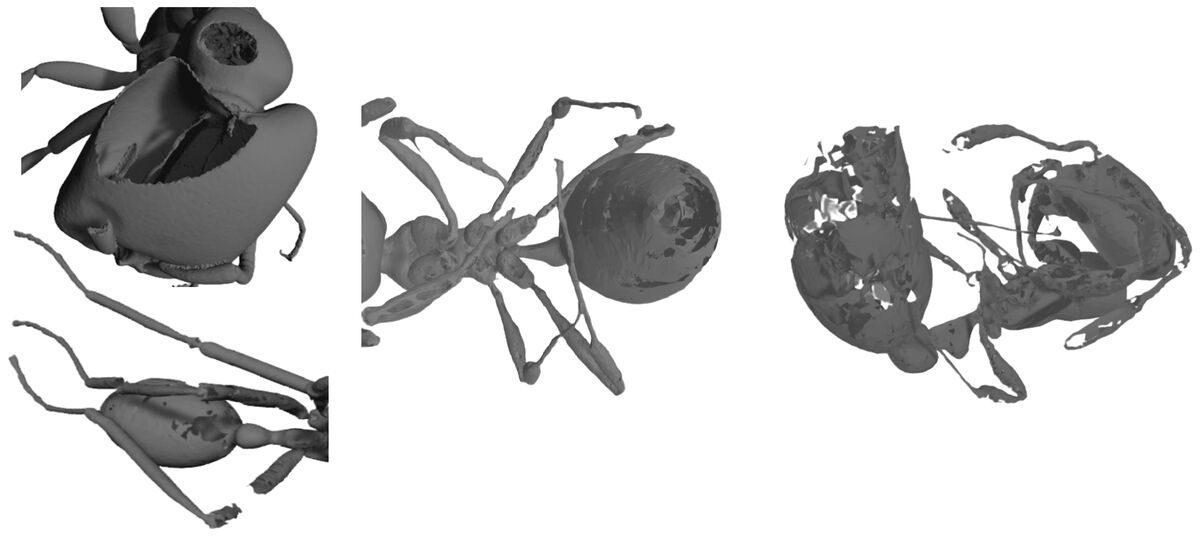
\includegraphics[width=0.6\linewidth]{figures/fig_before_registration.jpg}
\caption{Raw scans before registration: holes, self-intersections and
missing surface at exactly the structures of greatest anatomical interest:
the visual evidence motivating the brief's preprocessing-first
hypothesis.}
\label{fig:before-registration}
\end{figure}

The internship brief's implicit hypothesis was that input mesh quality was
the dominant bottleneck (Figure~\ref{fig:before-registration}). The first
weeks were spent building a unified preprocessing pipeline with explicit
diagnostics and quality classification, retained in the delivered system
because its outputs make later fitting decisions auditable.

\begin{investigation}{I2}{Does cleaner input produce more accurate registration?}
\invQuestion{Holding the registration stage fixed, does the rebuilt
preprocessing pipeline improve fit accuracy over the existing one?}
\invMethod{Head-to-head mean Chamfer distance across a matched specimen set,
new pipeline vs.\ existing pipeline, registration stage identical.}
\invResult{$0.000771$ (new) vs.\ $0.000737$ (existing), under five
percent apart, nominally \emph{favouring} the existing pipeline, and far too
small to account for the correspondence gap characterised in
\S\ref{sec:synthetic-instrument}.}
\invVerdict{REJECT}{Topology improved substantially (\S3.3) without moving
this surface metric, so mesh conditioning alone does not explain the
correspondence failures under investigation. This comparison uses Chamfer
distance as a coverage check, not an anatomical-correctness check
(\F{F1} shows the latter is unreliable); the claim is deliberately limited to
what Chamfer distance can support (coverage did not change), and
motivated testing whether the limitation lay downstream of mesh conditioning
instead. Recorded as \F{F2}.}
\end{investigation}

A clear improvement here would have justified further investment in
preprocessing; instead, the comparison ruled out mesh quality as the
dominant explanation and reframed the central question of the internship
from \emph{how clean is the input} to \emph{what determines whether the
optimiser finds the right correspondence at all}: the question the rest
of this chapter answers.
